\section*{Appendix}

\subsection*{Additional Tables and Figures}
\begin{table}[h!]
    \centering
    \caption{Summary Statistics of Financial Data}
    \begin{tabular}{|c|c|c|c|c|c|c|}
        \hline
        Security & Mean & Median & Std Dev & Min & Max & Volume \\
        \hline
        Stock A & 100 & 98 & 5 & 90 & 110 & 50000 \\
        Stock B & 50 & 49 & 3 & 45 & 55 & 30000 \\
        ... & ... & ... & ... & ... & ... & ... \\
        \hline
    \end{tabular}
\end{table}

\begin{figure}[h!]
    \centering
    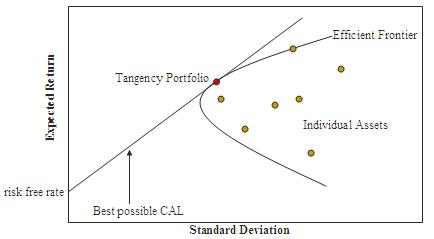
\includegraphics[width=\textwidth]{efficient_frontier.png}
    \caption{Efficient Frontier of Optimal Portfolios}
    \label{fig:efficient_frontier}
\end{figure}

\subsection*{Methodology Details}
This section provides detailed explanations of the methods used in the empirical analysis, including the mathematical formulations of the CAPM and Sharpe Ratio calculations, the steps involved in applying Modern Portfolio Theory (MPT), and the procedures for conducting Monte Carlo simulations.

\subsubsection*{CAPM Calculation}
The steps for calculating the CAPM for each security are as follows:
\begin{enumerate}
    \item Calculate the average return of the market index (e.g., S&P 500).
    \item Determine the risk-free rate (e.g., the yield on 10-year U.S. Treasury bonds).
    \item Compute the beta (\(\beta\)) of each security by regressing its returns against the market returns.
    \item Use the CAPM formula:
    \[ E(R_i) = R_f + \beta_i (E(R_m) - R_f) \]
    to estimate the expected return for each security.
\end{enumerate}

\subsubsection*{Sharpe Ratio Calculation}
The steps for calculating the Sharpe Ratio are:
\begin{enumerate}
    \item Calculate the expected return of each security using the CAPM.
    \item Determine the risk-free rate.
    \item Calculate the standard deviation of the excess return for each security.
    \item Use the Sharpe Ratio formula:
    \[ S = \frac{E(R_i) - R_f}{\sigma_i} \]
    to measure the risk-adjusted return of each security.
\end{enumerate}

\subsubsection*{Modern Portfolio Theory (MPT)}
The steps for applying MPT to construct and optimize portfolios are:
\begin{enumerate}
    \item Define the assets and their expected returns and covariances.
    \item Determine the weights of the assets in the portfolio to maximize the expected return for a given level of risk.
    \item Construct the efficient frontier to visualize the set of optimal portfolios.
\end{enumerate}

\subsubsection*{Monte Carlo Simulation Steps}
The steps for conducting Monte Carlo simulations are:
\begin{enumerate}
    \item Define the initial investment and annual contribution.
    \item Generate random returns based on historical data.
    \item Repeat the simulation multiple times to estimate the distribution of outcomes.
    \item Analyze the distribution of simulated outcomes to assess the probability of achieving the target down payment.
\end{enumerate}

\subsection*{Python Code Snippets}
\begin{verbatim}
# Example Python code for downloading data using Yahoo Finance API

import yfinance as yf
import pandas as pd

# List of securities
securities = ['AAPL', 'MSFT', 'GOOGL', 'TSLA', 'AMZN']

# Download historical data
data = yf.download(securities, start='2014-09-07', end='2024-09-07', interval='1d')

# Display the data
print(data.head())

# Example Python code for CAPM calculation

import numpy as np

def calculate_capm(returns, market_returns, risk_free_rate):
    beta = np.cov(returns, market_returns)[0, 1] / np.var(market_returns)
    expected_return = risk_free_rate + beta * (np.mean(market_returns) - risk_free_rate)
    return expected_return, beta

# Example Python code for Sharpe Ratio calculation

def calculate_sharpe_ratio(returns, risk_free_rate):
    excess_returns = returns - risk_free_rate
    return np.mean(excess_returns) / np.std(excess_returns)

# Example Python code for Modern Portfolio Theory (MPT)

def optimize_portfolio(returns):
    n = len(returns.columns)
    weights = np.random.random(n)
    weights /= np.sum(weights)
    
    portfolio_return = np.dot(weights, returns.mean())
    portfolio_risk = np.sqrt(np.dot(weights.T, np.dot(returns.cov(), weights)))
    
    return portfolio_return, portfolio_risk, weights

# Example Python code for Monte Carlo Simulation

def monte_carlo_simulation(portfolio_return, portfolio_risk, initial_investment, n_simulations, time_horizon):
    simulation_results = []
    for _ in range(n_simulations):
        portfolio_value = initial_investment
        for _ in range(time_horizon):
            portfolio_value *= (1 + np.random.normal(portfolio_return, portfolio_risk))
        simulation_results.append(portfolio_value)
    return simulation_results
\end{verbatim}
